\section{Design}
I dette projekt er der valgt så vidt muligt at designe alle løsninger med analog elektronik. Derfor er det valgt at forforstærkeren bygges af commonemittertrin med uafkoblet emittermodstand. Et commonemittertrins typiske opbygning er vist på figur \ref{fig:cekobling}.

\begin{figure}[h]
\centering
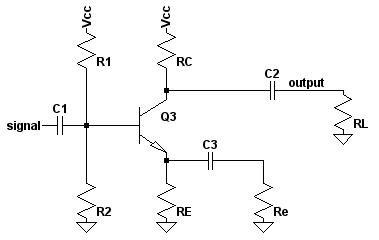
\includegraphics[scale=.6]{teknisk/forforstaerker/ceopkobling.png}
\caption{Generel form på commonemitterkobling med uafkoblet emittermodstand}
\label{fig:cekobling}
\end{figure}


Argumentet for dette valg er at det er det eneste trin, blandt commonemitter, -base og -collector, hvis spændingsforstærkning er betydeligt over én og ikke, under korrekte omstændigheder, afhænger af transistorparametre. Da transistorparametre blandt andet er afhængige af den anvendte transistors temperatur er det en betragtelig styrke ikke at skulle tage højde for dem. Spændingsforstærkningen i commonemittertrinnet er dog kun uafhængig af transistorparametre så længe følgende er gældende: $r_o >>R_C \| R_L$, $gm \cdot R_E||R_e$ og $i_e \approx i_c$.
Disse antagelser vil være gældende gennem hele designet af forforstærkeren. 
Forforstærkeren bygges af to commonemittertrin for at opnå den ønskede forstærkning på 63,3 gange. Dette skyldes at forstærkningen er givet ved ligning (\ref{eq:gmbevis})\fixme{kilde sedra smith eller mm6 AEL}.

\begin{equation}
A_v =  \frac{-gm \cdot R'_L}{1+gm \cdot R'_e} \approx  -\frac{R'_L}{R'_e} \Biggr\vert _{\frac{1}{gm}<R'_e}
\label{eq:gmbevis}
\end{equation}

Hvor $R'_e = R_e || R_E$ og $R'_L = R_L||R_C$. Det vil sige at jo tættere $R_e$ kommer på $\frac{1}{gm}$ jo mere indflydelse vil denne have på forstærkningen.

Det første trin skal have en forstærkning på 10 gange og det andet på 6,33 for at opnå den ønskede forstærkning, som vist på figur \ref{blok_forforstaerker}. Grunden til rækkefølgen af trinnene er for ikke at have størst signaludsving og den største forstærkning i samme trin.\fixme{Hvordan viser vi at det er smart?}

\begin{figure}[h]
\centering
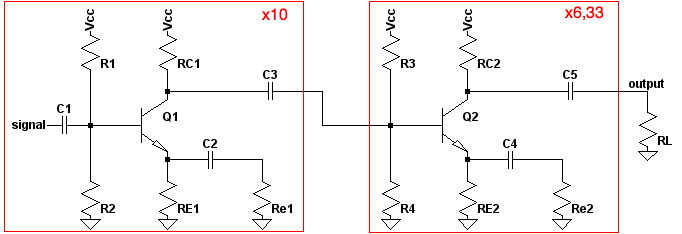
\includegraphics[scale=.6]{teknisk/forforstaerker/blok_forforstaerker.png}
\caption{Blokdiagram over forforstærkerens byggeblokke samt lydsignalets vej}
\label{blok_forforstaerker}
\end{figure}

For at opnå så lav forvrængning som muligt designes hvert trin således at forstærkningen, uden den AC-koblede emittermodstand $R_e$, er så stor som muligt for at gøre tilbagekobling muligt. For derefter at få den ønskede forstærkning tilføjes tilbagekoblingsmodstanden $R_e$.

\subsection*{Design af første trin}
Begge trin designes efter maksimal forstærkning uden $R_e$. Denne forstærkning er givet ved ligning (\ref{eq:dcgain}).

\begin{equation}
|A_{vs}|=\frac{1}{\left(\frac{V_t \cdot R_C}{V_{R_C}}+\frac{R'_S}{\beta}\right) \left(\frac{1}{R_C}+\frac{1}{R_L}\right)}
\label{eq:dcgain}
\end{equation}
Hvor $R'_S = R_S||R_1||R_2$ og $V_t = 26 \cdot 10^{-3}$.

For at designe et kredsløb med maksimal forstærkning justeres størrelsen af $R_C$ uden at variere spændingen over den, $V_{R_C}$. Den maksimale $R_C$ findes ved ligning \ref{eq:rcmaks}.

\begin{equation}
R_{\mathrm{C,maks}} = \sqrt{\frac{R'_S \cdot R_L \cdot V_{R_C}}{\beta \cdot V_t}}
\label{eq:rcmaks}
\end{equation}

I ligning \ref{eq:rcmaks} er $R'_S$ defineret som $R_1||R_2||R_S$. $R_S$ er fastlagt til 2,2 k\ohm, hvilket er mikrofonens udgangsimpedans\fixme{kilde til MCE4000}. Parallelforbindelsen mellem $R_1$ og $R_2$ kan ikke beregnes men skal vælges. Indgangsimpedansen i kredsløbet, som netop er $R_1||R_2$, skal som hovedregel være meget større end udgangsimpedansen i den kreds den belaster. En tommelfingerregel siger at 10 gange større er tilstrækkeligt til at være $"$meget større$"$ hvormed parallelkoblingen skal være over eller lig med 22 k\ohm. 
Belastningen, $R_L$, for det første trin bliver indgangsimpedansen i det andet. Indgangsimpedansen i det andet trin bliver $R_3||R_4$ og kan heller ikke beregnes. Da $R_C$ i det første trin ikke kendes endnu vælges indgangsimpedansen i det andet til at være den samme som i det første, altså 22 k\ohm. 
$V_{R_C}$ er defineret som værende $V_{CC} - V_{\mathrm{CE,sat}} - V_{R_E} - V_{\mathrm{o,peak}}$, hvor $V_{CC}$ vælges til 15 V så der sikres at der er plads til det ønskede spændingsudsving, $V_{R_E}$ vælges til 3 V og $V_{\mathrm{CE,sat}}$ aflæses i databladet for BC547b til 0,2 V ved en collectorstrøm på 1 mA. Der antages at collectorstrømmen cirka bliver 1 mA. Ligeledes aflæses $\beta$ til 250 ved 1 mA i databladet. $V_{\mathrm{o,peak}}$ er peakspændingen på udgangen. Dermed bliver peakspændingen en faktor 10 højere end mikrofonens output peakspænding. $V_{\mathrm{o,peak}}$ bliver derfor 316 mV. $R_C1$ beregnes hermed i ligning (\ref{eq:rcforsteberegning}).

\begin{equation}
R_{\mathrm{C1}} = \sqrt{\frac{22~k\ohm || 2,2~k\ohm \cdot (15~V - 0,2~V - 3~V - 0,316~V)}{250 \cdot 26 \cdot 10^{-3}}}=8,82~k\ohm
\label{eq:rcforsteberegning}
\end{equation}

$R_{E1}$ bestemmes i ligning \ref{eq:beregningre1} under antagelse at $i_e = i_c$. 

\begin{equation}
i_c=\frac{V_{R_C}}{R_C}=\frac{11,5~V}{9,25~k\ohm}=106,4~mA
\end{equation}
\begin{equation}
R_{E1}=\frac{V_{R_{E1}}}{\frac{V_{R_{C1}}}{R_{C1}}}  \Rightarrow R_{E1}=\frac{3~V}{106,4~mA}=2,30~k\ohm
\label{eq:beregningre1}
\end{equation}


Dernæst beregnes $R_e1$ ud fra hvad den ønskede forstærkning skal være. Ligning (\ref{eq:gmbevis}) benyttes til at beregne $R_e1$ i ligning (\ref{eq:rlilleeberegning}).

\begin{equation}
A_v = -\frac{R'_L}{R'_e} \Rightarrow  R_{e1} =-\frac{R_L \cdot R_{C1} \cdot R_{E1}}{A_v \cdot R_{E1} \cdot R_{C1} + A_v \cdot R_{E1} \cdot R_L + R_{C1} \cdot R_L} \Rightarrow R_{e1} = 866,18~\ohm
\end{equation}

Biasnetværket, bestående af $R_1$ og $R_2$ beregnes ud fra den spænding, som er påkrævet på basen for at transistoren fungerer som ønsket. Spændingen over base-emitter, $V_{\mathrm{BE}}$ er i databladet aflæst til 0,6 V. Da potentialet på emitteren er 3 V skal potentialet på basen være 3,6 V. $R_1$ og $R_2$ kan beregnes ud fra at $V_{R_2}$ skal være 3,6 V og parallelkoblingen $R_1||R_2$. Beregningen udføres i ligning (\ref{eq:r1r21}) og (\ref{eq:r1r22}).

\begin{equation}
V_{R_2} = V_{CC} \cdot \frac{R_2}{R_1+R_2} 
\label{eq:r1r21}
\end{equation}
\begin{equation}
R_1||R_2 = \frac{R_1 \cdot R_2}{R_1 + R_2}
\label{eq:r1r22}
\end{equation}
De kendte værdier indsættes og de to ligninger med to ubekendte løses. Resultatet er vist i ligning \ref{eq:r1r2result}.
\begin{equation}
R_1 = 91,7~k\ohm ~ \wedge ~ R_2=28,9~k\ohm
\label{eq:r1r2result}
\end{equation}



\subsection*{Design af andet trin}
Beregning af andet trin følger samme procedure som første trin. Beregningerne kan findes i appendiks ?? \fixme{kilde appendiks}
Modstands- og kondensatorværdier samt ændrede betingelser er vist i tabel \ref{tab:trintovalues}.

\begin{table}[h]
\centering
\begin{tabular}{l|r}
\hline\hline
$R_L$ & 30,8 k$\omega$ \\
\hline\hline
Forstærkning & 63,3 gange \\[4pt]
Forvrængning & < 0,5 \% \\[4pt]
Indgangsimpedans & > 5 k\ohm \\
\hline\hline
\end{tabular}
\caption{Krav til forforstærkeren}
\label{tab:krav_forforstaerker}
\end{table}


